\documentclass[aspectratio=169,10pt]{beamer}
\usepackage[T1]{fontenc}
\usepackage{amsmath,amssymb,amsfonts}
\usepackage{bm}
\usepackage{tikz}
\usepackage{xcolor}
\usetikzlibrary{arrows.meta,positioning,shapes,calc}

\definecolor{parchment}{HTML}{F4E8C8}
\definecolor{paper}{HTML}{FAF1D8}
\definecolor{ink}{HTML}{1A1A1A}
\definecolor{inkgray}{HTML}{5A5A5A}
\definecolor{accentred}{HTML}{8B1A1A}
\definecolor{accentgreen}{HTML}{2D5F2C}
\definecolor{accentblue}{HTML}{1F4E79}
\definecolor{redbg}{HTML}{F7E0DE}
\definecolor{grnbg}{HTML}{E0EBDC}
\definecolor{blubg}{HTML}{DDE6EF}
\definecolor{labelbg}{HTML}{EFE0B0}

\usefonttheme{serif}
\setbeamercolor{background canvas}{bg=parchment}
\setbeamercolor{normal text}{fg=ink}
\setbeamercolor{structure}{fg=ink}
\setbeamercolor{frametitle}{fg=ink,bg=parchment}
\setbeamercolor{title}{fg=ink}
\setbeamercolor{itemize item}{fg=ink}
\setbeamercolor{itemize subitem}{fg=ink}
\setbeamercolor{item}{fg=ink}
\setbeamercolor{caption name}{fg=ink}
\setbeamertemplate{navigation symbols}{}
\setbeamertemplate{itemize item}{\textbullet}

\setbeamertemplate{frametitle}{%
  \vspace{0.30em}%
  \begin{center}%
    {\bfseries\Large\insertframetitle\par}%
    \vspace{0.28em}%
    {\color{ink}\rule{0.86\paperwidth}{0.4pt}}%
  \end{center}%
  \vspace{0.10em}%
}
\setbeamertemplate{footline}{%
  \hbox to \paperwidth{\hfil\itshape\small\insertframenumber\hspace{0.7em}}%
  \vspace{0.35em}%
}

\newcommand{\vY}{\bm{Y}}
\newcommand{\vy}{\bm{y}}
\newcommand{\vA}{\bm{A}}
\newcommand{\vB}{\bm{B}}
\newcommand{\valpha}{\bm{\alpha}}
\newcommand{\vn}{\bm{n}}
\newcommand{\vs}{\bm{s}}
\newcommand{\vW}{\bm{W}}
\newcommand{\T}{^{\mathsf T}}
\newcommand{\Hh}{^{\mathsf H}}
\newcommand{\norm}[1]{\left\lVert #1\right\rVert}
\DeclareMathOperator*{\argmin}{arg\,min}

\tikzset{
  flowbox/.style={draw=ink,fill=paper,line width=0.6pt,
                  minimum width=2.5cm,minimum height=1.0cm,
                  align=center,font=\small\bfseries,inner sep=4pt},
  smallbox/.style={draw=ink,fill=paper,line width=0.4pt,
                   minimum width=0.7cm,minimum height=0.55cm,
                   inner sep=2pt,align=center,font=\footnotesize\itshape},
  method/.style={draw=accentgreen,fill=grnbg,line width=1.0pt,
                 align=center,font=\small\bfseries,inner sep=6pt},
  issue/.style={draw=accentred,fill=redbg,line width=1.0pt,
                align=center,font=\small\bfseries,inner sep=6pt},
  idea/.style={draw=accentblue,fill=blubg,line width=1.0pt,
               align=center,font=\small\bfseries,inner sep=6pt},
  flowarr/.style={-{Stealth[length=2.5mm,width=2mm]},line width=0.7pt},
  softarr/.style={-{Stealth[length=2mm,width=1.6mm]},line width=0.5pt,color=inkgray}
}

\newcommand{\bottomnote}[1]{%
  \begin{center}{\itshape\small #1}\end{center}}

\newcommand{\papercover}[4]{%
  \begin{frame}[plain]
    \vfill
    \begin{center}
      {\bfseries\Huge #1\par}
      \vspace{0.8cm}
      {\Large #2\par}
      \vspace{0.35cm}
      {\itshape\large\color{inkgray}#3\par}
      \vspace{0.55cm}
      {\small\texttt{\detokenize{#4}}\par}
    \end{center}
    \vfill
  \end{frame}}

\newcommand{\twocolmodel}[4]{%
  \begin{columns}[T,onlytextwidth]
    \begin{column}{0.48\textwidth}#1\end{column}
    \begin{column}{0.48\textwidth}#2\end{column}
  \end{columns}
  \bottomnote{#3\\#4}}


\usetikzlibrary{fit,decorations.pathreplacing}

\newcommand{\jj}{\mathrm{j}}
\newcommand{\Kset}{\mathcal K}
\newcommand{\Bset}{\mathcal B}
\newcommand{\C}{\mathbb C}

\tikzset{
  card/.style={draw=ink,fill=paper,line width=0.55pt,rounded corners=2pt,
               align=center,inner sep=5pt,font=\small},
  goodcard/.style={draw=accentgreen,fill=grnbg,line width=0.85pt,
                   rounded corners=2pt,align=center,inner sep=5pt,font=\small},
  badcard/.style={draw=accentred,fill=redbg,line width=0.85pt,
                  rounded corners=2pt,align=center,inner sep=5pt,font=\small},
  bluecard/.style={draw=accentblue,fill=blubg,line width=0.85pt,
                   rounded corners=2pt,align=center,inner sep=5pt,font=\small},
  ghostcard/.style={draw=inkgray!65,fill=paper,line width=0.55pt,dashed,
                    rounded corners=2pt,align=center,inner sep=5pt,
                    font=\small,text=inkgray},
  matrixcell/.style={draw=inkgray!65,line width=0.25pt,
                     minimum width=0.36cm,minimum height=0.36cm,
                     inner sep=0pt},
  redarr/.style={-{Stealth[length=2.5mm,width=2mm]},line width=0.85pt,
                  draw=accentred},
  greenarr/.style={-{Stealth[length=2.5mm,width=2mm]},line width=0.85pt,
                    draw=accentgreen},
  bluearr/.style={-{Stealth[length=2.5mm,width=2mm]},line width=0.85pt,
                   draw=accentblue},
  cpbrace/.style={decorate,decoration={brace,amplitude=5pt,raise=2pt},
                  line width=0.6pt,color=inkgray}
}

\begin{document}

% =====================================================================
% 1. Cover
% =====================================================================
\begin{frame}[plain]
  \centering
  \vspace{0.25cm}
  {\small\color{inkgray}Intercarrier interference (ICI) and intersymbol interference (ISI)\par}
  \vspace{0.20cm}
  {\bfseries\Huge ICI and ISI\par}
  \vspace{0.25cm}
  {\Large Doppler, insufficient cyclic prefix, and\par
   joint demodulation and decoding\par}
  \vspace{0.55cm}

  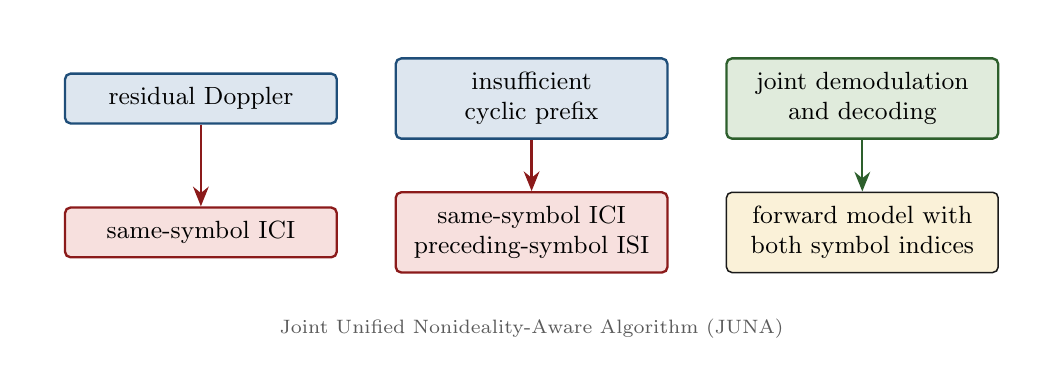
\begin{tikzpicture}[x=1cm,y=1cm]
    \path[use as bounding box] (-6.4,-2.2) rectangle (6.4,1.8);
    \node[bluecard,text width=3.1cm] (dop) at (-4.2,0.9)
      {residual Doppler};
    \node[badcard,text width=3.1cm] (ici) at (-4.2,-0.8)
      {same-symbol ICI};
    \draw[redarr] (dop) -- (ici);

    \node[bluecard,text width=3.1cm] (cp) at (0,0.9)
      {insufficient cyclic prefix};
    \node[badcard,text width=3.1cm] (both) at (0,-0.8)
      {same-symbol ICI\\preceding-symbol ISI};
    \draw[redarr] (cp) -- (both);

    \node[goodcard,text width=3.1cm] (joint) at (4.2,0.9)
      {joint demodulation\\and decoding};
    \node[card,text width=3.1cm] (model) at (4.2,-0.8)
      {forward model with\\both symbol indices};
    \draw[greenarr] (joint) -- (model);
    \node[font=\scriptsize\color{inkgray}] at (0,-2.02)
      {Joint Unified Nonideality-Aware Algorithm (JUNA)};
  \end{tikzpicture}
\end{frame}

% =====================================================================
% 2. Cyclic prefix
% =====================================================================
\begin{frame}{Cyclic prefix}
  \centering
  {\small Orthogonal Frequency Division Multiplexing (OFDM) symbol;
   cyclic prefix (CP)\par}
  \vspace{0.25cm}
  \begin{tikzpicture}[x=1cm,y=1cm,>=Stealth]
    \path[use as bounding box] (-6.5,-2.6) rectangle (6.5,2.5);

    \draw[->,line width=0.65pt] (-6.2,0) -- (6.2,0)
      node[right,font=\scriptsize] {time};
    \draw[fill=paper,draw=ink] (-6.0,0.25) rectangle (-2.0,1.05);
    \node[font=\small] at (-4.0,0.65) {preceding useful interval};

    \draw[fill=blubg,draw=accentblue,line width=0.9pt]
      (-2.0,0.25) rectangle (-0.7,1.05);
    \node[font=\small] at (-1.35,0.65) {prefix};

    \draw[fill=grnbg,draw=accentgreen,line width=0.9pt]
      (-0.7,0.25) rectangle (5.6,1.05);
    \node[font=\small] at (2.45,0.65) {current useful interval};

    \only<2->{
      \draw[bluearr] (4.4,1.20)
        .. controls (3.1,2.25) and (-0.9,2.25) .. (-1.35,1.20);
      \node[font=\scriptsize\color{accentblue}] at (1.45,2.13)
        {copy the final samples};
      \draw[accentblue,line width=2.0pt] (4.4,1.15) -- (5.55,1.15);
    }

    \only<3->{
      \draw[cpbrace] (-1.9,-0.25) -- (-0.7,-0.25);
      \node[font=\scriptsize] at (-1.3,-0.70) {cyclic-prefix length $L_{\rm cp}$};
      \draw[accentgreen,line width=3.2pt] (-1.72,-1.35) -- (-0.7,-1.35);
      \node[font=\scriptsize\color{accentgreen},anchor=east] at (-1.85,-1.35)
        {channel memory $L_h-1$};
      \draw[greenarr] (-0.7,-1.75) -- (5.55,-1.75);
      \node[font=\scriptsize\color{accentgreen}] at (2.4,-2.12)
        {fast Fourier transform window};
    }
  \end{tikzpicture}
  \vspace{-0.15cm}
  \bottomnote{An adequate prefix contains the channel memory before the useful interval begins.}
\end{frame}

% =====================================================================
% 3. One-tap model
% =====================================================================
\begin{frame}{One-tap model}
  \begin{columns}[T,onlytextwidth]
    \begin{column}{0.47\textwidth}
      \centering
      {\small Fast Fourier transform (FFT)\par}
      \vspace{0.25cm}
      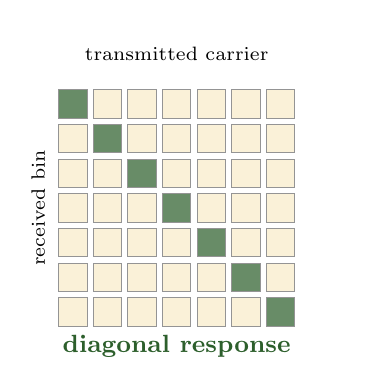
\begin{tikzpicture}[x=0.44cm,y=0.44cm]
        \path[use as bounding box] (-1.3,-1.4) rectangle (7.8,8.2);
        \foreach \r in {0,...,6}{
          \foreach \c in {0,...,6}{
            \node[matrixcell,fill=paper] at (\c,6-\r) {};
          }
          \node[matrixcell,fill=accentgreen!72] at (\r,6-\r) {};
        }
        \node[font=\scriptsize] at (3,7.45) {transmitted carrier};
        \node[font=\scriptsize,rotate=90] at (-1.0,3) {received bin};
        \node[font=\small\bfseries\color{accentgreen}] at (3,-1.0)
          {diagonal response};
      \end{tikzpicture}
    \end{column}
    \begin{column}{0.51\textwidth}
      \vspace{0.65cm}
      \[
        \mathbf Y_s=\mathbf H_s\mathbf X_s+\bm\nu_s,
        \qquad \mathbf H_s\ \text{diagonal}.
      \]
      \vspace{0.25cm}
      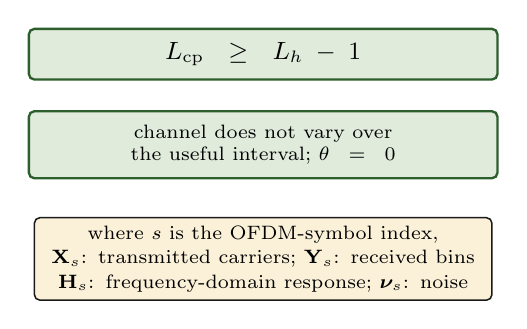
\begin{tikzpicture}
        \node[goodcard,text width=5.6cm] at (0,1.05)
          {$L_{\rm cp}\ge L_h-1$};
        \node[goodcard,text width=5.6cm,font=\scriptsize] at (0,-0.10)
          {channel does not vary over the useful interval; $\theta=0$};
        \node[card,text width=5.6cm,font=\scriptsize,inner sep=3pt] at (0,-1.55)
          {where $s$ is the OFDM-symbol index,\\[0.1em]
           $\mathbf X_s$: transmitted carriers; $\mathbf Y_s$: received bins\\[0.1em]
           $\mathbf H_s$: frequency-domain response; $\bm\nu_s$: noise};
      \end{tikzpicture}
    \end{column}
  \end{columns}
  \bottomnote{\scriptsize Under both conditions, one channel gain acts on each carrier.}
\end{frame}

% =====================================================================
% 4. Residual Doppler
% =====================================================================
\begin{frame}{Residual Doppler}
  \centering
  \begin{tikzpicture}[x=1cm,y=1cm,>=Stealth]
    \path[use as bounding box] (-6.4,-2.8) rectangle (6.4,2.9);

    \begin{scope}[shift={(-3.8,0.55)}]
      \draw[inkgray] (-1.45,0) -- (1.45,0);
      \draw[inkgray] (0,-1.45) -- (0,1.45);
      \draw[accentgreen,line width=1.4pt,domain=0:360,samples=120]
        plot ({1.15*cos(\x)},{1.15*sin(\x)});
      \fill[accentgreen] (1.15,0) circle (2pt);
      \node[font=\small\bfseries\color{accentgreen}] at (0,-1.92)
        {closed loop};
      \node[font=\scriptsize] at (0,1.90) {$q\ne k,\ a=0,\ \theta=0$};
    \end{scope}

    \only<2->{
      \begin{scope}[shift={(3.8,0.55)}]
        \draw[inkgray] (-1.45,0) -- (1.45,0);
        \draw[inkgray] (0,-1.45) -- (0,1.45);
        \draw[accentred,line width=1.4pt,domain=0:444.6,samples=150]
          plot ({1.15*cos(\x)},{1.15*sin(\x)});
        \fill[accentred] ({1.15*cos(444.6)},{1.15*sin(444.6)}) circle (2pt);
        \draw[redarr,line width=1.1pt] (0,0) -- (0.32,0.29);
        \node[font=\small\bfseries\color{accentred}] at (0,-1.92)
          {unfinished loop};
        \node[font=\scriptsize] at (0,1.90) {$\Delta_{4,5}=1.235$};
        \node[font=\scriptsize\color{accentred},anchor=west]
          at (0.40,0.38) {time average $H_{4,5}$};
      \end{scope}
    }

    \only<3->{
      \node[bluecard,text width=8.7cm] at (0,-2.25) {%
        $\displaystyle
        \Delta_{k,q}=(q-k)+\theta+aq$\\[0.15em]
        \scriptsize where $q$ is the carrier, $k$ is the bin,
        $a$ is the residual Doppler factor, and $\theta$ is carrier frequency offset};
    }
  \end{tikzpicture}
\end{frame}

% =====================================================================
% 5. Carrier coupling
% =====================================================================
\begin{frame}{Carrier coupling}
  \centering
  \vspace{-0.18cm}
  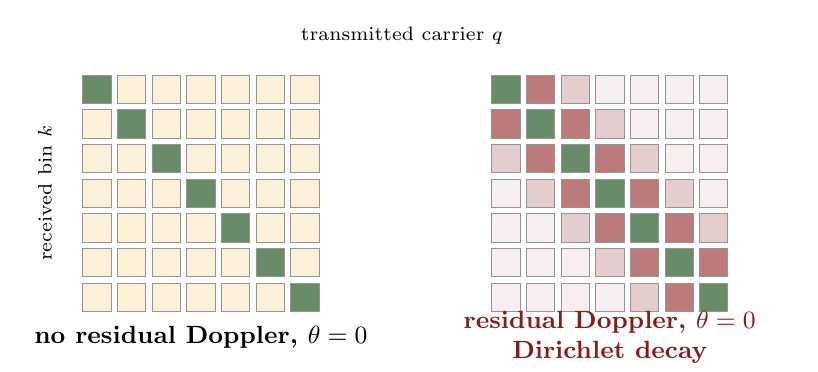
\begin{tikzpicture}[x=0.44cm,y=0.44cm]
    \path[use as bounding box] (-7.5,-1.35) rectangle (14.5,7.78);

    \begin{scope}[shift={(-5.5,0)}]
      \foreach \r in {0,...,6}{
        \foreach \c in {0,...,6}{
          \node[matrixcell,fill=paper] at (\c,6-\r) {};
        }
        \node[matrixcell,fill=accentgreen!72] at (\r,6-\r) {};
      }
      \node[font=\small\bfseries,align=center] at (3,-1.15)
        {no residual Doppler, $\theta=0$};
    \end{scope}

    \only<2->{
      \begin{scope}[shift={(6.3,0)}]
        \foreach \r in {0,...,6}{
          \foreach \c in {0,...,6}{
            \pgfmathtruncatemacro{\dist}{abs(\r-\c)}
            \ifnum\dist=0
              \node[matrixcell,fill=accentgreen!72] at (\c,6-\r) {};
            \else\ifnum\dist=1
              \node[matrixcell,fill=accentred!58] at (\c,6-\r) {};
            \else\ifnum\dist=2
              \node[matrixcell,fill=accentred!22] at (\c,6-\r) {};
            \else
              \node[matrixcell,fill=accentred!7] at (\c,6-\r) {};
            \fi\fi\fi
          }
        }
        \node[font=\small\bfseries\color{accentred},align=center] at (3,-1.15)
          {residual Doppler, $\theta=0$\\Dirichlet decay};
      \end{scope}
    }

    \node[font=\scriptsize] at (3.3,7.55) {transmitted carrier $q$};
    \node[font=\scriptsize,rotate=90] at (-7.0,3) {received bin $k$};
  \end{tikzpicture}

  \vspace{-0.15cm}
  \only<3->{
    \[
      Y_{k,s}=H_{k,k,s}X_{k,s}
      +\sum_{q\ne k}H_{k,q,s}X_{q,s}+\nu_{k,s}.
    \]
    \centering\scriptsize
    where $H_{k,q,s}$ is the response and $\nu_{k,s}$ is noise.
  }
  \only<3->{
    \centering\scriptsize
    Same symbol index, different carrier index: ICI.\\
    The coefficients have Dirichlet decay; the receiver retains a banded approximation.\par
  }
\end{frame}

% =====================================================================
% 6. Insufficient cyclic prefix
% =====================================================================
\begin{frame}{Insufficient cyclic prefix}
  \centering
  \begin{tikzpicture}[x=1cm,y=1cm,>=Stealth]
    \path[use as bounding box] (-6.5,-2.7) rectangle (6.5,2.6);

    \draw[->,line width=0.65pt] (-6.2,0) -- (6.2,0)
      node[right,font=\scriptsize] {time};
    \draw[fill=paper,draw=ink] (-6.0,0.30) rectangle (-2.0,1.10);
    \node[font=\small] at (-4.0,0.70) {preceding useful interval};
    \draw[fill=blubg,draw=accentblue,line width=0.9pt]
      (-2.0,0.30) rectangle (-0.7,1.10);
    \node[font=\small] at (-1.35,0.70) {prefix};
    \draw[fill=grnbg,draw=accentgreen,line width=0.9pt]
      (-0.7,0.30) rectangle (5.6,1.10);
    \node[font=\small] at (2.45,0.70) {current useful interval};

    \draw[accentred,line width=3.2pt] (-2.65,-0.75) -- (-0.05,-0.75);
    \node[font=\scriptsize\color{accentred},anchor=east] at (-2.78,-0.75)
      {channel memory $L_h-1$};
    \draw[cpbrace] (-2.0,-1.25) -- (-0.7,-1.25);
    \node[font=\scriptsize,anchor=east] at (-1.48,-1.72) {$L_{\rm cp}$};

    \only<2->{
      \fill[accentred!32] (-0.7,0.30) rectangle (-0.05,1.10);
      \draw[accentred,line width=1.0pt] (-0.7,0.30) rectangle (-0.05,1.10);
      \draw[redarr] (-3.0,1.45)
        .. controls (-2.5,2.15) and (-0.4,2.15) .. (-0.30,1.20);
      \node[font=\scriptsize\color{accentred}] at (-1.55,2.13)
        {preceding-symbol tail};
      \node[font=\scriptsize\color{accentred}] at (-0.38,0.70) {$D$};
    }

    \only<3->{
      \node[badcard,text width=6.7cm] at (2.75,-1.85) {%
        $\displaystyle D=\min\!\left\{N,\max(0,L_h-1-L_{\rm cp})\right\}$\\[0.1em]
        $\displaystyle\text{contaminated fraction}=\frac{D}{N}$};
    }
  \end{tikzpicture}
  \bottomnote{\scriptsize where $N$ is the useful-interval length,
  $L_h-1$ is the channel memory, and $L_{\rm cp}$ is the prefix length;
  this diagram has $L_h-1\le L_{\rm cp}+N$.
  A tap beyond the prefix carries the preceding symbol into the useful interval.}
\end{frame}

% =====================================================================
% 7. Symbol indices
% =====================================================================
\begin{frame}{Symbol indices}
  \centering
  \begin{tikzpicture}[x=1cm,y=1cm,>=Stealth]
    \path[use as bounding box] (-6.4,-2.44) rectangle (6.4,2.8);
    \node[card,text width=2.3cm] (prev) at (-4.7,0.95)
      {preceding symbol\\$\mathbf X_{s-1}$};
    \node[goodcard,text width=2.3cm] (curr) at (-4.7,-0.65)
      {current symbol\\$\mathbf X_s$};
    \node[ghostcard,text width=2.3cm] (next) at (-4.7,-1.82)
      {following symbol\\$\mathbf X_{s+1}$};
    \node[bluecard,text width=2.3cm] (out) at (4.8,-0.35)
      {received bins\\$\mathbf Y_s$};

    \draw[greenarr] (curr) -- node[above,font=\scriptsize] {$\mathbf H_0$} (out);
    \only<2->{
      \draw[redarr] (prev) -- node[above,font=\scriptsize] {$\mathbf J_-$} (out);
    }
    \only<3->{
      \draw[softarr,dashed] (next) -- node[below,font=\scriptsize] {$\mathbf J_+$} (out);
      \node[font=\scriptsize\color{inkgray},align=center] at (1.0,-2.08)
        {causal channel; FFT window aligned with useful interval:\\
         $\mathbf J_+=\mathbf 0$};
    }

    \only<4->{
      \node[card,text width=9.5cm] at (0,2.35) {%
        $\displaystyle
        \mathbf Y_s=\mathbf H_0\mathbf X_s
        +\mathbf J_-\mathbf X_{s-1}
        +\mathbf J_+\mathbf X_{s+1}+\bm\nu_s$};
    }
  \end{tikzpicture}
  \vspace{-0.15cm}
  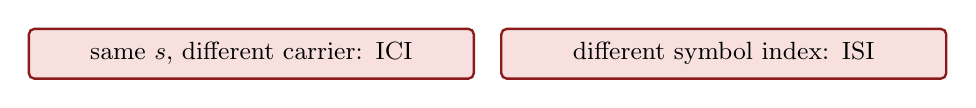
\begin{tikzpicture}
    \node[badcard,text width=5.3cm] at (-3.0,0)
      {same $s$, different carrier: ICI};
    \only<2->{\node[badcard,text width=5.3cm] at (3.0,0)
      {different symbol index: ISI};}
  \end{tikzpicture}
  \bottomnote{\scriptsize where $\mathbf H_0$ is the same-symbol response,
  $\mathbf J_-$ and $\mathbf J_+$ are adjacent-symbol responses,
  and $\bm\nu_s$ is noise.}
\end{frame}

% =====================================================================
% 8. Two conditions
% =====================================================================
\begin{frame}{Two conditions}
  \centering
  \begin{tikzpicture}[x=1cm,y=1cm]
    \path[use as bounding box] (-6.3,-3.1) rectangle (6.3,3.0);

    \node[goodcard,text width=4.7cm] at (-3.0,2.15)
      {prefix contains channel memory\\$L_{\rm cp}\ge L_h-1$};
    \node[goodcard,text width=4.7cm] at (3.0,2.15)
      {channel does not vary\\over useful interval; $\theta=0$};

    \node[font=\small\bfseries] at (-4.95,1.15) {prefix};
    \node[font=\small\bfseries] at (-1.65,1.15) {channel ($\theta=0$)};
    \node[font=\small\bfseries] at (2.15,1.15) {frequency-domain result};

    \node[card,text width=2.25cm] at (-4.95,0.30) {adequate};
    \node[card,text width=2.25cm] at (-1.65,0.30) {does not vary};
    \node[goodcard,text width=4.2cm] at (2.15,0.30) {one-tap model};

    \only<2->{
      \node[card,text width=2.25cm] at (-4.95,-0.65) {adequate};
      \node[badcard,text width=2.25cm] at (-1.65,-0.65)
        {residual Doppler};
      \node[badcard,text width=4.2cm] at (2.15,-0.65) {same-symbol ICI};
    }

    \only<3->{
      \node[badcard,text width=2.25cm] at (-4.95,-1.60) {insufficient};
      \node[card,text width=2.25cm] at (-1.65,-1.60) {does not vary};
      \node[badcard,text width=4.2cm] at (2.15,-1.60)
        {same-symbol ICI\\preceding-symbol ISI};
    }

    \only<4->{
      \node[badcard,text width=2.25cm] at (-4.95,-2.55) {insufficient};
      \node[badcard,text width=2.25cm] at (-1.65,-2.55)
        {residual Doppler};
      \node[badcard,text width=4.2cm,font=\scriptsize,inner sep=3pt] at (2.15,-2.55)
        {same-symbol ICI from both causes\\plus preceding-symbol ISI};
    }
  \end{tikzpicture}
\end{frame}

% =====================================================================
% 9. JUNA model
% =====================================================================
\begin{frame}{JUNA model}
  \centering
  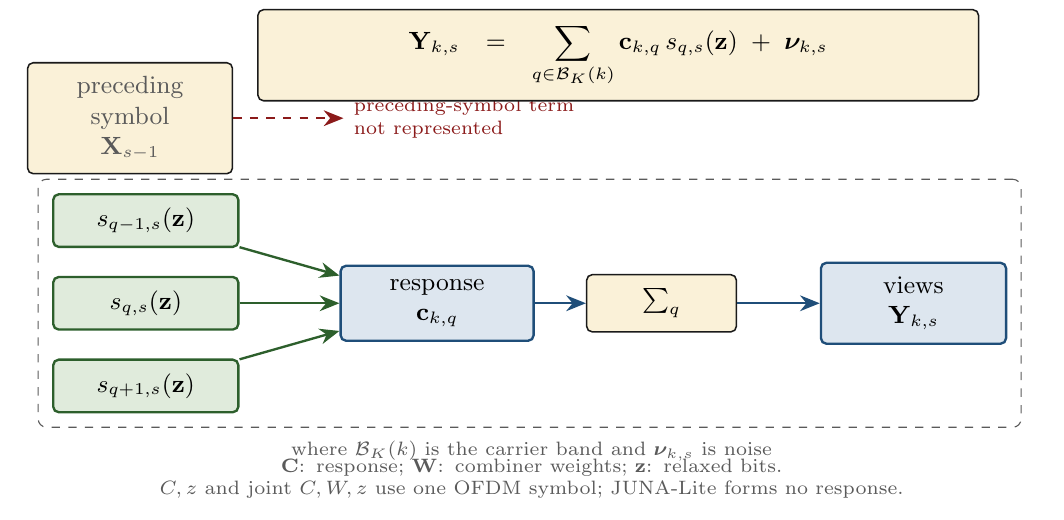
\begin{tikzpicture}[x=1cm,y=1cm,>=Stealth]
    \path[use as bounding box] (-6.4,-3.0) rectangle (6.4,2.9);

    \only<2->{
      \node[card,text=inkgray,text width=2.25cm] (previous) at (-5.1,1.75)
        {preceding\\symbol\\$\mathbf X_{s-1}$};
    }

    \node[goodcard,text width=2.0cm] (q1) at (-4.9,0.45)
      {$s_{q-1,s}(\mathbf z)$};
    \node[goodcard,text width=2.0cm] (q2) at (-4.9,-0.60)
      {$s_{q,s}(\mathbf z)$};
    \node[goodcard,text width=2.0cm] (q3) at (-4.9,-1.65)
      {$s_{q+1,s}(\mathbf z)$};
    \node[bluecard,text width=2.1cm] (resp) at (-1.2,-0.60)
      {response\\$\mathbf c_{k,q}$};
    \node[card,text width=1.55cm] (sum) at (1.65,-0.60) {$\sum_q$};
    \node[bluecard,text width=2.0cm] (obs) at (4.85,-0.60)
      {views\\$\mathbf Y_{k,s}$};

    \draw[greenarr] (q1) -- (resp);
    \draw[greenarr] (q2) -- (resp);
    \draw[greenarr] (q3) -- (resp);
    \draw[bluearr] (resp) -- (sum);
    \draw[bluearr] (sum) -- (obs);

    \only<2->{
      \draw[redarr,dashed] (previous.east) -- ++(1.4,0)
        node[right,font=\scriptsize\color{accentred},align=left]
        {preceding-symbol term\\not represented};
    }

    \node[draw=inkgray,dashed,rounded corners=3pt,fit=(q1)(q2)(q3)(resp)(sum)(obs),
          inner sep=5pt] {};
    \node[font=\scriptsize\color{inkgray}] at (0,-2.48)
      {where $\mathcal B_K(k)$ is the carrier band and $\bm\nu_{k,s}$ is noise};
    \node[font=\scriptsize\color{inkgray},align=center,text width=11.2cm] at (0,-2.83)
      {$\mathbf C$: response; $\mathbf W$: combiner weights;
       $\mathbf z$: relaxed bits.\\
       $C,z$ and joint $C,W,z$ use one OFDM symbol;
       JUNA-Lite forms no response.};

    \node[card,text width=8.8cm] at (1.1,2.55) {%
      $\displaystyle
      \mathbf Y_{k,s}=\sum_{q\in\Bset_K(k)}
      \mathbf c_{k,q}\,s_{q,s}(\mathbf z)+\bm\nu_{k,s}$};
  \end{tikzpicture}
\end{frame}

% =====================================================================
% 10. Audience question
% =====================================================================
\begin{frame}[plain]
  \vfill
  \begin{center}
    {\bfseries\Huge Can joint demodulation\\[0.25em]
    and decoding solve both?}
  \end{center}
  \vfill
\end{frame}

% =====================================================================
% 11. Joint objective
% =====================================================================
\begin{frame}{Joint objective}
  \centering
  \begin{tikzpicture}[x=1cm,y=1cm,>=Stealth]
    \path[use as bounding box] (-6.3,-2.9) rectangle (6.3,3.0);

    \node[bluecard,text width=2.55cm] (obs) at (-4.7,1.30)
      {received\\observations\\$\mathbf Y$};
    \node[goodcard,text width=2.55cm] (bits) at (-4.7,-0.65)
      {relaxed coded\\bits\\$\mathbf z$};
    \node[bluecard,text width=2.55cm] (response) at (-1.1,1.30)
      {response\\$\bm\psi$};
    \node[card,text width=2.55cm] (symbols) at (-1.1,-0.65)
      {symbols\\$\mathbf s(\mathbf z)$};
    \node[bluecard,text width=2.7cm] (like) at (2.7,1.30)
      {observation likelihood};
    \only<2->{
      \node[goodcard,text width=2.7cm] (parity) at (2.7,-0.65)
        {parity constraints};
    }

    \draw[bluearr] (obs.south east)
      .. controls (-2.8,0.42) and (0.8,0.42) .. (like.south west);
    \draw[bluearr] (response) -- (like);
    \draw[greenarr] (bits) -- (symbols);
    \draw[bluearr] (symbols) -- (like);
    \only<2->{\draw[greenarr] (bits) -- (parity);}

    \node[card,text width=11.0cm] at (0,2.55) {%
      $\displaystyle
      \mathcal L(\bm\psi,\mathbf z)
      =-\log p\!\left(\mathbf Y\mid\mathbf s(\mathbf z),\bm\psi\right)
       -\log p(\bm\psi)
       \only<2->{+\lambda_{\rm p}\mathcal R_{\rm par}(\mathbf z)}$};

    \only<3->{
      \node[badcard,text width=7.5cm] at (0,-2.02)
        {A channel contribution omitted from the likelihood\\cannot be cancelled explicitly.};
    }
    \node[font=\scriptsize,align=center,text width=11.5cm] at (0,-2.72)
      {where $\bm\psi$ contains the response parameters
       \only<2->{and $\lambda_{\rm p}$ weights the parity penalty
       $\mathcal R_{\rm par}$}.};
  \end{tikzpicture}
\end{frame}

% =====================================================================
% 12. Adjacent symbols
% =====================================================================
\begin{frame}{Adjacent symbols}
  \centering
  \begin{tikzpicture}[x=1cm,y=1cm,>=Stealth]
    \path[use as bounding box] (-6.3,-2.82) rectangle (6.3,3.0);

    \only<2->{
      \node[badcard,text width=2.6cm] (prev) at (-4.8,0.85)
        {preceding carriers\\$s_{q,s-1}(\mathbf z)$};
    }
    \node[goodcard,text width=2.6cm] (curr) at (-4.8,-0.90)
      {current carriers\\$s_{q,s}(\mathbf z)$};
    \node[bluecard,text width=2.7cm] (resp) at (-0.8,-0.05)
      {\alt<2->{same-symbol and\\preceding-symbol\\response}
                 {same-symbol\\response}};
    \node[bluecard,text width=2.4cm] (out) at (4.55,-0.05)
      {received views\\$\mathbf Y_{k,s}$};

    \only<2->{
      \draw[redarr] (prev.east) --
        node[above,pos=0.35,font=\scriptsize] {$r=s-1$} (resp.north west);
    }
    \draw[greenarr] (curr.east) --
      node[below,pos=0.35,font=\scriptsize] {$r=s$} (resp.south west);
    \draw[bluearr] (resp) -- (out);

    \only<3->{
      \node[goodcard,text width=3.8cm] (code) at (0,-1.65)
        {parity constraints on $\mathbf z$};
    }

    \node[card,text width=11.2cm] at (0,2.45) {%
      \alt<2->{%
        $\displaystyle
        \mathbf Y_{k,s}
        =\sum_{(q,r)\in\Bset(k,s)}
         \mathbf c_{k,s;q,r}\,s_{q,r}(\mathbf z)+\mathbf n_{k,s}$%
      }{%
        $\displaystyle
        \mathbf Y_{k,s}
        =\sum_{q\in\Bset_K(k)}
         \mathbf c_{k,q}\,s_{q,s}(\mathbf z)+\mathbf n_{k,s}$%
      }};
    \node[font=\small\itshape,align=center,text width=11.8cm] at (0,-2.48)
      {\alt<2->{%
        where $\mathcal B(k,s)$ contains the represented carrier and symbol indices
        and $\mathbf n_{k,s}$ is noise.\\
        Modeling extension, not a CP-short experiment.%
      }{%
        where $\mathcal B_K(k)$ is the carrier band and $\mathbf n_{k,s}$ is noise%
      }\only<3->{\\Parity applies within the same codeword.}};
  \end{tikzpicture}
\end{frame}

% =====================================================================
% 13. Receiver requirements
% =====================================================================
\begin{frame}{Receiver requirements}
  \centering
  \begin{tikzpicture}[x=1cm,y=1cm]
    \path[use as bounding box] (-6.3,-3.0) rectangle (6.3,3.0);

    \only<1->{\node[bluecard,text width=3.4cm,minimum height=1.15cm]
      at (-4.1,1.65) {channel memory\\and cyclic-prefix length};}
    \only<1->{\node[bluecard,text width=3.4cm,minimum height=1.15cm]
      at (0,1.65) {FFT-window\\alignment};}
    \only<2->{\node[bluecard,text width=3.4cm,minimum height=1.15cm]
      at (4.1,1.65) {neighboring OFDM-symbol\\observations};}
    \only<2->{\node[goodcard,text width=3.4cm,minimum height=1.15cm]
      at (-4.1,-0.15) {pilots across\\neighboring symbols};}
    \only<3->{\node[goodcard,text width=3.4cm,minimum height=1.15cm]
      at (0,-0.15) {carrier and\\symbol support};}
    \only<3->{\node[goodcard,text width=3.4cm,minimum height=1.15cm]
      at (4.1,-0.15) {parity\\constraints};}

    \only<4->{
      \node[badcard,text width=10.6cm] at (0,-2.05)
        {The measured results do not validate a CP-relaxation rule.};
    }
  \end{tikzpicture}
\end{frame}

% =====================================================================
% 14. Two receiver paths
% =====================================================================
\begin{frame}
  \centering
  \begin{tikzpicture}[x=1cm,y=1cm,>=Stealth]
    \path[use as bounding box] (-6.3,-3.0) rectangle (6.3,3.0);

    \node[badcard,text width=5.2cm] (cause) at (0,2.35)
      {cyclic-prefix length\\compared with channel memory};

    \node[goodcard,text width=4.2cm] (adequate) at (-3.5,0.85)
      {adequate cyclic prefix};
    \only<2->{
      \node[bluecard,text width=4.2cm] (short) at (3.5,0.85)
        {insufficient cyclic prefix};
    }
    \draw[greenarr] (cause) -- (adequate);
    \only<2->{\draw[bluearr] (cause) -- (short);}

    \node[card,text width=4.2cm] (current) at (-3.5,-0.40)
      {$\mathbf J_-=\mathbf0$\\same-symbol response\\one-tap or residual-Doppler ICI};
    \only<2->{
      \node[card,text width=4.2cm] (extended) at (3.5,-0.40)
        {$\mathbf H_0\mathbf X_s+\mathbf J_-\mathbf X_{s-1}$\\same-symbol response and\\preceding-symbol response};
    }
    \draw[greenarr] (adequate) -- (current);
    \only<2->{\draw[bluearr] (short) -- (extended);}

    \only<3->{
      \node[card,text width=11.0cm,font=\scriptsize] at (0,-2.38)
        {The current response can represent the same-symbol term;
         the preceding-symbol term requires the modeling extension.\\
         JUNA-Lite assumes an adequate prefix and forms no response.\\
         For no residual Doppler, the useful-symbol duration is sufficiently
         shorter than the channel coherence time.};
    }
  \end{tikzpicture}
\end{frame}

% =====================================================================
% 15. Takeaways
% =====================================================================
\begin{frame}{Takeaways}
  \centering
  \vspace{0.35cm}
  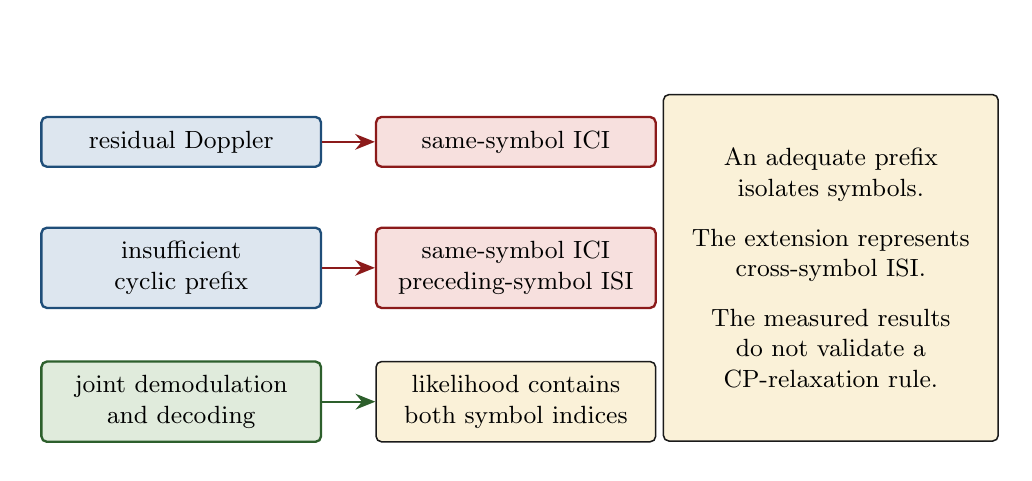
\begin{tikzpicture}[x=1cm,y=1cm,>=Stealth]
    \path[use as bounding box] (-6.2,-2.7) rectangle (6.2,2.7);

    \node[bluecard,text width=3.2cm] (dop) at (-4.25,1.25)
      {residual Doppler};
    \node[badcard,text width=3.2cm] (ici) at (0,1.25)
      {same-symbol ICI};
    \draw[redarr] (dop) -- (ici);

    \node[bluecard,text width=3.2cm] (cp) at (-4.25,-0.35)
      {insufficient cyclic prefix};
    \node[badcard,text width=3.2cm] (isi) at (0,-0.35)
      {same-symbol ICI\\preceding-symbol ISI};
    \draw[redarr] (cp) -- (isi);

    \node[goodcard,text width=3.2cm] (joint) at (-4.25,-2.05)
      {joint demodulation\\and decoding};
    \node[card,text width=3.2cm] (need) at (0,-2.05)
      {likelihood contains\\both symbol indices};
    \draw[greenarr] (joint) -- (need);

    \node[card,text width=3.9cm,minimum height=4.4cm,font=\small] at (4.00,-0.35)
      {An adequate prefix\\isolates symbols.\\[0.75em]
       The extension represents\\cross-symbol ISI.\\[0.75em]
       The measured results\\do not validate a\\CP-relaxation rule.};
  \end{tikzpicture}
\end{frame}

\end{document}
